% Copied this sample latex file from https://www.usenix.org/conferences/author-resources/paper-templates
\documentclass[letterpaper,twocolumn,11pt]{article}
\usepackage{usenix,epsfig,endnotes}
\usepackage{array}
\usepackage[usenames, dvipsnames]{color}

\newcolumntype{L}[1]{>{\raggedright\let\newline\\\arraybackslash\hspace{0pt}}m{#1}}
\newcolumntype{C}[1]{>{\centering\let\newline\\\arraybackslash\hspace{0pt}}m{#1}}
\newcolumntype{R}[1]{>{\raggedleft\let\newline\\\arraybackslash\hspace{0pt}}m{#1}}

\usepackage{helvet}
\renewcommand{\familydefault}{\sfdefault}

\begin{document}

%don't want date printed
\date{}

%make title bold and 14 pt font (Latex default is non-bold, 16 pt)
\title{\Large \bf Kaggle Challenge: Predicting Rossmann Store Sales}

\author{
  {\rm Min Gu Jo}\\
  University of California, Berkeley
  \and
      {\rm Wonjohn Choi}\\
      University of California, Berkeley
} % end author

\maketitle

% Use the following at camera-ready time to suppress page numbers.
% Comment it out when you first submit the paper for review.
\thispagestyle{empty}


\section{Abstract}
Our project attempted to apply linear regression and various machine learning techniques to a real-world problem of predicting drug store sales. Rossmann, Germany's second-largest drug store chain, has provided past sales information of 1115 Rossmann stores located across Germany. We preprocessed, feature-engineered the data, and examined 3 different statistical / machine learning analysis for forecasting sales of each store: multivariate linear regression with various feature selection methods, Random Forest regression, and Gradient Boosting with regression trees. Then, we compared the methods' predictive power by computing Root Mean Square Percentage Error (RMSPE). We found that Gradient Boosting model performed the best with a RMSPE score of 0.13234 on the test data set.

\section{Introduction}
The objective of this project is to predict 6 weeks of daily sales for 1115 Rossmann stores located across Germany using the data which was provided by Rossmann through Kaggle. The motivation of this project is the following: by reliably predicting daily sales, store managers may decrease operational costs, and create effective staff schedules (ex. by assigning more staffs during busy days) (``Rossmann Store Sales''). Also, we would like to identify which type of techniques are both efficient and effective in a real-world sales prediction task. Before building any regression or machine learning models for the prediction, we attempted to identify which features in the data might be significant to determine daily sales of stores, and investigate any interesting relationships between variables.

To start off, we first explored several similar efforts that made for sales prediction task in the past in order to set the basis of our study, and reviewed them to discover how we can improve for our regression task. 

    Linear Regression: The professor at Western Illinois University suggests multiple linear regression with various feature selection methods and multicollinearity diagnostics to be a popuplar technique in sales forecasting. This model was applied for predicting the number of subscribers that a cable station can expect, which is closely related to our task (Dehkordi-Vakil). However, her features in her dataset for her regression task were only 5 compared to our 20. Also, she didn't engineer her features much, while some of our features required one hot encoding to extract more informations and increase dimensions of our dataset. Therefore, compared to her, we decided to apply several various feature selection methods such as partial t-test and stepwise regression to select significant features. 

    Random Forest: Random Forest is a tree-based ensemble method where all trees depend on a collection of random variables. (Breiman). Breiman, UC Berkeley professor, suggested that Random Forest algorithm is actually from a classification viewpoint but the approach is applicable to regression as well (Breiman). Therefore, we consider the Random Forest is also applicable to our sales prediction task. For a similar apporach, Nils Adriansson and Ingrid Mattsson in their thesis applies the Random Forest into a GDP forecast task, showing its power in time-series forecasting (Adriansson). However, for the train set, they had only 58 observations compared to our ${~1,000,000}$. To make our computation faster, we chose to use ``H2O'' library which enables parallelized computation although Adriansson could easily use R's Random Forest for his smaller dataset. We assume this algorithm would outperform linear regression because Breiman states that the Random Forest does not need to assume any distribution for variables (Breiman).

    Gradient Boosting: We also found an useful article by Jay Gu, PhD in Machine Learning from Carnegie Mellon University, on gradient boosting regression. In his article, he asserted that, for predictive analytics, the gradient boosted tree model (GBM) is one of the most effective machine learning models (Gu). As he did, we have also witnessed a good number of winning solutions for various kaggle competitions that contain boosted tree models as a crucial component. To set the basic framework of Gradient Boosting, we reviewed Tianqi Chen's presentation (Chen). In Gu's ``Bike Sharing classification prediction'', we witnessed that Gu reduced his computation time efficiently by dividing out certain features to seperately train boosting models. He later combined the predictions of these models to calculate weighted sums for his binary classification (Gu). We consider that his seperate training of models might enforce him to also tune hyperparameters seperately which would worsen his runtime efficiency. For our regression task, since we have to direcly predict the number of sales, we decided to not seperately train Gradient Boosting models, but increase our time efficieny by using R's `XGBoost` library to perform parallelized computation which enables faster cross validations for more hyperparameter tuning. 

\subsection{Description of Datasets}
Data sets are given by Rossmann through Kaggle. There are three files: ``test.csv'', ``train.csv'', and ``store.csv''. ``train.csv'' contains 1017209 observed daily sales of different stores from 2013 to 2015. ``store.csv'' contains supplementary information for each store (41088 lines because there are 41088 stores). ``train.csv'' and ``store.csv'' both contain Store id that we can use to join the train and store data sets. Finally, ``test.csv'' has 41088 lines of daily sales of different stores but the value of Sales column is omitted. We are expected to predict the value of Sales column for the test set (``test.csv'') by using the training set (``train.csv'') and store data (``store.csv'') (``Rossmann Store Sales'').

\newpage
The following table describes fields in ``test.csv'' and ``training.csv'':

\begin{tabular}{| c | L{5cm} |}
  \hline
  Store & the unique id for each store (positive integer ranging from 1 to 1115) \\ \hline
  DayOfWeek & the day of week (positive integer ranging from 1 to 7 where 1, 2, ..., 7 correspond to Monday, Tuesday, ..., Sunday) \\ \hline
  Date & the date (string of format YYYY­MM­DD) \\ \hline
  Sales & the total amount of revenue for this given day (positive number between 0 and 41551). This value is what needs to be predicted, so only exists in ``training.csv''. \\ \hline
  Customers & the number of customers on the given day. This also only exists in ``training.csv''. \\ \hline
  Open & an indicator of whether the store was open on the given day (0 if closed, 1 if open) \\ \hline
  Promo & an indicator of whether the store was running a promotion on the given day (0 if not running, 1 if running) \\ \hline
  StateHoliday & an indicator of whether the given day was a state holiday (0 if not a state holiday, a if public holiday, b if eastern holiday, c if christmas) \\ \hline
  SchoolHoliday & an indicator of whether the store was affected by a nearby school holiday on the given day (0 if not affected, 1 if affected) \\ \hline
\end{tabular}


\newpage
The following table describes fields in ``store.csv'':

\begin{tabular}{| L{2cm} | L{5cm} |}
  \hline
  Store & the unique id for each store (positive integer ranging from 1 to 1115) \\ \hline
  StoreType & the store's model (4 types: a, b, c, d) \\ \hline
  CompetitionDistance & the distance in meters to the nearest competing store (positive number ranging from 20.0 to 75860.0, and NA's if no competitors) \\ \hline
  Competition OpenSince Month & the approximate month of the time when the nearest competing store opened (positive integer ranging from 1 to 12, and NA's if no competitors) \\ \hline
  Competition OpenSince Year & the approximate year of the time when the nearest competing store opened (positive integer ranging from 1900 to 2015, and NA's if no competitors) \\ \hline
  Assortment & the store's assortment level (a = basic, b = extra, c = extended) \\ \hline
  Promo2 & an indicator of whether the store was participating in a promotion that runs over a period of time  (0 if not participating, 1 if participating) \\ \hline
  Promo2 SinceWeek & the approximate week of year when the store started to participate in promo2 (positive integer ranging from 1 to 50, and NA's if no promo2) \\ \hline
  Promo2 SinceYear & the approximate year of time when the store started to participate in promo2 (positive integer ranging from 2009 to 2015, and NA's if no promo2) \\ \hline
\end{tabular}

\section{Methods}
We first performed preprocessing the raw data given by Rossmann.

\subsection{Preprocessing}
For preprocessing, we have done the followings:
\begin{itemize}
\item We first merged ``train.csv'' and ``store.csv'' by ``Store'' because we can predict daily sales better with more data related to the sales. We also merged ``test.csv'' and ``store.csv'' by ``Store''. Then, We removed ``Customers'' field from the training data because it does not exist in the test data so we cannot use ``Customers'' to predict ``Sales''.
\item For ``CompetitionDistance'' with NA values, we replaced NA with 1000000. Since 1000000 is much more bigger than any other distances, replacing NA with the number simulated an effect of having no competitor. In the similar way, we filled missing values for ``CompetitionOpenSinceYear'' and ``CompetitionOpenSinceMonth''. Similarly, for ``Promo2SinceYear'' with NA valus, we replaced NA with 1990 to simulate the effect of having no promo2.
\item We splitted ``Date'' field into three fields: ``year'', ``month'', and ``day'' to better account for the effects each components of date have.
\item We computed average sales for each store to create a new field ``Average.Sales''. This variable seemed to be an indicator of how well a store will perform in future. This makes sense because a store with a strong past performance is likely to perform well in future.
\item  We noticed the feature ``CompetitionDistance'' is highly skewed to right. For the sake of linear regression, we took log transformation on the feature ``CompetitionDistance'' to create a new field ``LogCompetitionDistance'' to make sure that the relationship between explanatory variables and dependent variable is approximately linear.
\end{itemize}

\textit{Our R codes for preprocessing are in ``Section A: Pre-processing'' of the supplementary file ``final-project.R''.}

\subsection{EDA (Exploratory Data Analysis)}
To check any distinctive relationships between variables before applications of prediction models, we drew a pearson correlation coefficient plot using R corrplot library. In the plot, we witnessed several interesting behaviors. We decided to explore deeper on the features: ``DayOfWeek'' and ``CompetitionDistance''.
\begin{enumerate}
\item ``DayOfWeek'' and ``Sales'' are negatively correlated. This implies that, as ``DayOfWeek'' approaches to Sunday, sales would decrease because drugstores would mostly close on Sunday.
  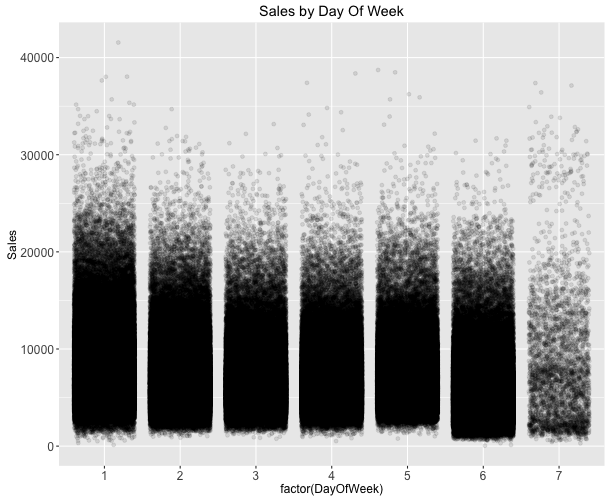
\includegraphics[scale=0.3]{img/sales_dayofweek.png}
\item ``LogCompetitionDistance'' and ``Sales'' are negatively correlated. In other words, lower distance to the competitor implies slightly higher sales. We assume this could occur because stores with a close distance to the competitor are mostly located in crowded regions such as a downtown city with higher sales overall. To check this pattern, we drew a scatterplot of average sales by competitiondistance.
  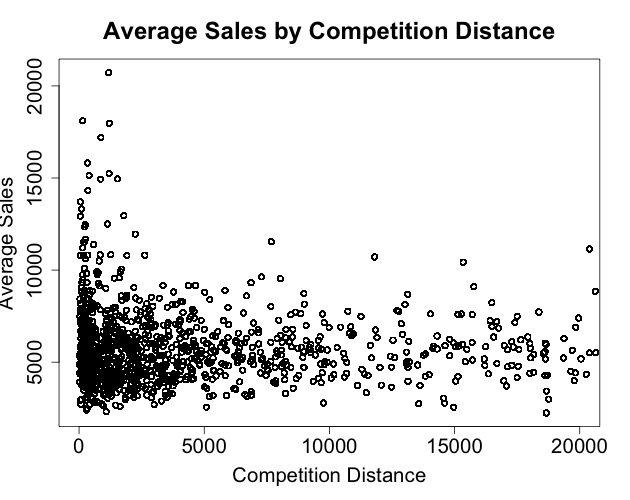
\includegraphics[scale=0.32]{img/compDist.png}
\end{enumerate}

\textit{Our R codes for EDA are in ``Section B: EDA'' of the supplementary file ``final-project.R''.}

\subsection{5-fold Cross Validation}
To generalize our predictions to limit problems of overfitting on the training set, we decided to ramdomly partition the original training observations into 5 equal sized subsamples. The training set is comprised of 4 equal sized subsamples and the rest as the validation set. For the purpose of reproducibility and comparison of the predictive powers of different models, we set the seed (with a value of 42). Our general process would be as the following:
\begin{enumerate}
\item  Repeat cross-validation process 5 times with each of the 5 subsamples used exactly once as the validation set.
\item Compute the average of 5 different validation error rate. 
\item Predict sales on the test set using the model. 
\item Submit on Kaggle website to get the test error rate.
\item Compare the average validation error rate and the test error rate among differnent models.
\end{enumerate}
  
\textit{Our R codes for 5-fold cross validation are in ``Section D: Cross Validation'' of the supplementary file ``final-project.R''.}

\subsection{Error Metric}
As the metrics that Kaggle uses to compute test error is the Root Mean Squared Percentage Error (RMSPE), we used the same metrics to compute our validation error. It's the following:

$RMSPE = \sqrt{\frac{1}{n} \sum {(\frac{y_i - \hat y_i}{y_i})}^2}$

where ${y_i}$ is a store's sales on a single day, ${yhat_i}$ is the daily sales prediction for the store on the day, and ${n}$ is the number of (store, date) pairs in the data set.

\textit{Our R codes used to compute error rates are in ``Section C: Utility Functions'' of the supplementary file ``final-project.R''.}

\subsection{Benchmark}
We started off by setting a benchmark to obtain a baseline for the prediction. Then, we took 3 different approaches to outperform the benchmark and former model.

Our benchmark is simply the average sales of each store. It is intuitive to predict daily sales of a store for a day with the average daily sales of a corresponding store. This method does not take account for many factors (whether the day was holiday, whether the store was running a promotion on the day, etc); thus, we expect its error rate to be higher than any other methods we applied.

\textit{Our R codes for benchmark are in ``Section E: Benchmark'' of the supplementary file ``final-project.R''.}

\subsection{Linear Regression}
Linear regression is an approach for modeling the relationship between dependent variable Y (in our case, ``Sales'') and explanatory variables X. To apply linear regression on the data, we decided to use R's $lm$ function. $lm$ is an implemention of multivariate linear regression. If we supply $Y \sim X$ as the input, $lm$ builds and returns a model that can be used to predict $Y$ using $X$. Under the hood, it basically solves the normal equation $\beta = (X^T X)^{-1} X^T Y$.

We first built linear model with all available features (``DayOfWeek'', ``Open'', ``Promo'', ``StateHoliday'', ``SchoolHoliday'', ``StoreType'', ``Assortment'', ``CompetitionOpenSinceMonth'', ``CompetitionOpenSinceYear'', ``Promo2'', ``Promo2SinceYear'', ``Average.Sales'', ``LogCompetitionDistance'', ``CompetitionDistance'', ``day'', ``month'', ``year'') using the training set. Then, we applied the linear model on validation set.

\textit{Our R codes for linear regression are in ``Section F: Linear Model'' of the supplementary file ``final-project.R''.}

\subsubsection{Feature Selection}
Then, we selected significant features to reduce complexity of the linear model. Beforehand, we took a look at the resulting lm with R function $summary(lm)$ to get some general idea of how important each variable is. Especially, we paid attention on partial t-test results (t-statistics) on the table. All features except ``CompetitionDistance'', ``CompetitionOpenSinceMonth'', ``CompetitionOpenSinceYear'', ``Promo2'', ``Promo2SinceYear'' were significant with p-value less than 0.05.

\subsubsection{Feature Selection-Backward Elimination}
Then, we applied backward elimination by repeatedly removing features with the highest p-value until no feature has p-value higher than 0.05. As the result, we obtained ``DayOfWeek'', ``Open'', ``Promo'', ``StateHoliday'', ``SchoolHoliday'', ``StoreType'', ``Assortment'', ``Average.Sales'', ``LogCompetitionDistance'', ``day'', ``month'', ``year''. Then, we built a linear model with the selected variables using the training set and performed prediction on the validation set.

\textit{Our R codes for linear regression with backward elimination are in ``Section G: Variable Selection-Backward Elimination'' of the supplementary file ``final-project.R''.}

\subsubsection{Feature Selection-Akaike Information Criterion}
Another approach we attempted for feature selection was using Akaike information criterion (AIC). AIC provides a measure of relative quality of models with the equation $AIC = 2k - 2 ln(L)$ where $k$ is the number of estimated paramters in the model and $L$ is the value of likelihood function. We performed AIC by using R function $stepAIC$ (Mazerolle).

\textit{Our R codes for linear regression with AIC are in ``Section H: Variable Selection-AIC'' of the supplementary file ``final-project.R''.}

\subsection{Random Forest}
Random Forest is an ensemble learning method that constructs decisions tree using training set. By aggregating many decision trees, Random Forest can make predictions while avoiding overfitting because it uses an ensemble of regression trees over different samples of the data (Breiman). Here is our Random Forest Regression steps: \\
\begin{enumerate}
\item Construct random forest regression trees (number of trees is defined by hyper parameter)
\item Classify the incoming data into the decision tree node
\item Calculate the mean value for each node for prediction
\end{enumerate}

In particular, we used H2O’s RandomForest package to carry out the training and prediction. Then, we optimized parameters to improve on our prediction model. H2O is the open source math engine for huge dataset (Aiello). Since H2O package enables us to compute Random Forest Regression algorithm in parallel distribution, we decided to use the package for faster computation compared to R's Random Forest package.

To find the best hyperparamters, we tried different values of hyperparamters, and compared the results on validation sets using cross validation steps.

\textit{Our R codes for random forest are in ``Section I: Random Forest'' of the supplementary file ``final-project.R''.}

\subsection{Gradient Boosting}
The similarity between Random Forest and Gradient Boosting is that both generate decision trees. However, Random forest uses bootstrapping method for training while Gradient Boosting builds decision tree over the residuals. In other words, Gradient Boosting Tree generates the decision tree as it optimizes on a proper loss function (Chen). This refers that we can establish our own loss function for optimization, while we couldn't do in Random Forest. We set our loss function to be our error metric, RMPSE. Our decision trees here are regression trees. Each regression tree divides the data point at each non-leaf node according to a constraint on a feature. The leaf node value of a data point decides its score, and a data point is predicted by averaging the scores of the leaf node it belongs to.

In particular, we used R's xgboost package. XGBoost also known as Extreme Gradient Boosting is a powerful supervised learning algorithm (Chen). This package enables an automatic parallel computation on a single machine. For our regression task, we put ``reg:linear'' for our objective function. 


\textit{Our R codes for gradient boosting are in ``Section J: Gradient Boosting'' of the supplementary file ``final-project.R''.}

\section{Supplementary Methods}
For anyone who would like to reproduce the results in this paper, we provided datasets and R codes we used in tar file ``supplementary-methods.tar.gz''.

To untar this tar file, please run the following command: ``tar xvfz supplementary-methods.tar.gz''.

This tar file should contain ``final-project.R'', ``data/store.csv'', ``data/test.csv'', and ``data/train.csv''.

``final-project.R'' contains all R codes used in this project, and it is referenced many time in ``Methods'' section of this paper. All files under folder ``data/'' are described in ``Description of Datasets'' subsection in ``Introduction'' section of this paper.

\section{Results}
\subsection{Benchmark}
Our benchmark is the average sales of each store. The error rate for benchmark was 0.106209 on the validation set and 0.25789 on the test set (when submitted to Kaggle website). This is our baseline model. Our goal is to improve our prediction by outperforming the benchmark by large degree at the end. 

\subsection{Linear Model}
The error rates of our different linear models on validation and test sets are the following:

\begin{center}
    \begin{tabular}{| l | l | l |}
      \hline
       & Validation & Test \\ \hline
      Linear Regression \\
      (Full Model) & 0.09101 & 0.21036 \\ \hline
      Linear Regression \\
      (Backward Elimination) & 0.09108 & 0.20988 \\ \hline
      Linear Regression \\
      (AIC) & 0.091006 & 0.21039 \\ \hline
      \hline    
    \end{tabular}
\end{center}

Through feature selection, we found that the following features ``CompetitionDistance'', ``CompetitionOpenSinceMonth'', ``CompetitionOpenSinceYear'', ``Promo2'', ``Promo2SinceYear'' were insignificant. This is evident in the following chart generated using output from R code $summary(lm_{all})$ where $lm_{all}$ is the linear model using all features (\textit{the code used here can be found in ``Section F: Linear Model'' of the supplementary file ``final-project.R''}):

\begin{center}
    \begin{tabular}{| l | l | l |}
      \hline
       & abs(t value) \\ \hline
      Average.Sales & 1071.340 \\ \hline
      Promo1 & 484.769 \\ \hline
      Open & 281.084 \\ \hline
      DayOfWeek & 215.891 \\ \hline
      month & 188.381 \\ \hline
      day & 70.741 \\ \hline
      year & 56.911 \\ \hline
      StateHoliday & 46.968 \\ \hline
      StoreType & 40.631 \\ \hline
      SchoolHoliday & 34.476 \\ \hline
      Assortment & 5.091 \\ \hline
      LogCompetitionDistance & 4.823 \\ \hline 
      Promo2SinceWeek & 4.436 \\ \hline
      \textcolor{red}{Promo2SinceYear} & 1.785 \\ \hline  
      \textcolor{red}{CompetitionOpenSinceMonth} & 2.208 \\ \hline
      \textcolor{red}{Promo2} & 1.369 \\ \hline
      \textcolor{red}{CompetitionOpenSinceYear} & 1.183 \\ \hline
      \textcolor{red}{CompetitionDistance} & 0.528 \\ \hline
      \hline    
    \end{tabular}
\end{center}

In the above chart, features with low abs(t-value) are marked with red. They have p-value more than 0.05 so are insignificant.

\subsection{Random Forest}
The major parameters we tune for Random Forest are the depth and number of trees. We used 5 fold cross validation to compute average RMSPE while varying the depth and number of trees. The learning curve for increasing depth is shown below:

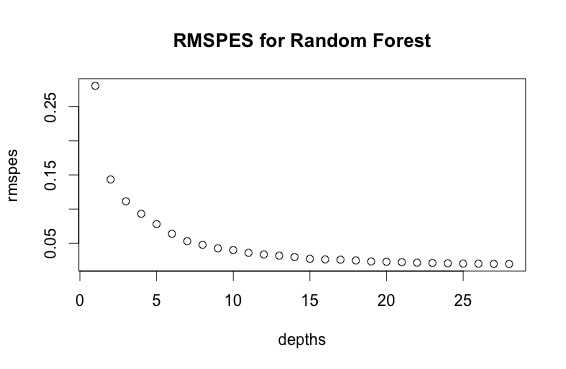
\includegraphics[scale=0.4]{img/RandomForestPerDepth.png}

As the curve illustrates, we see that RMSPE does not change much after the depth of trees reaches 20.

The learning curve for increasing ntrees is shown below:

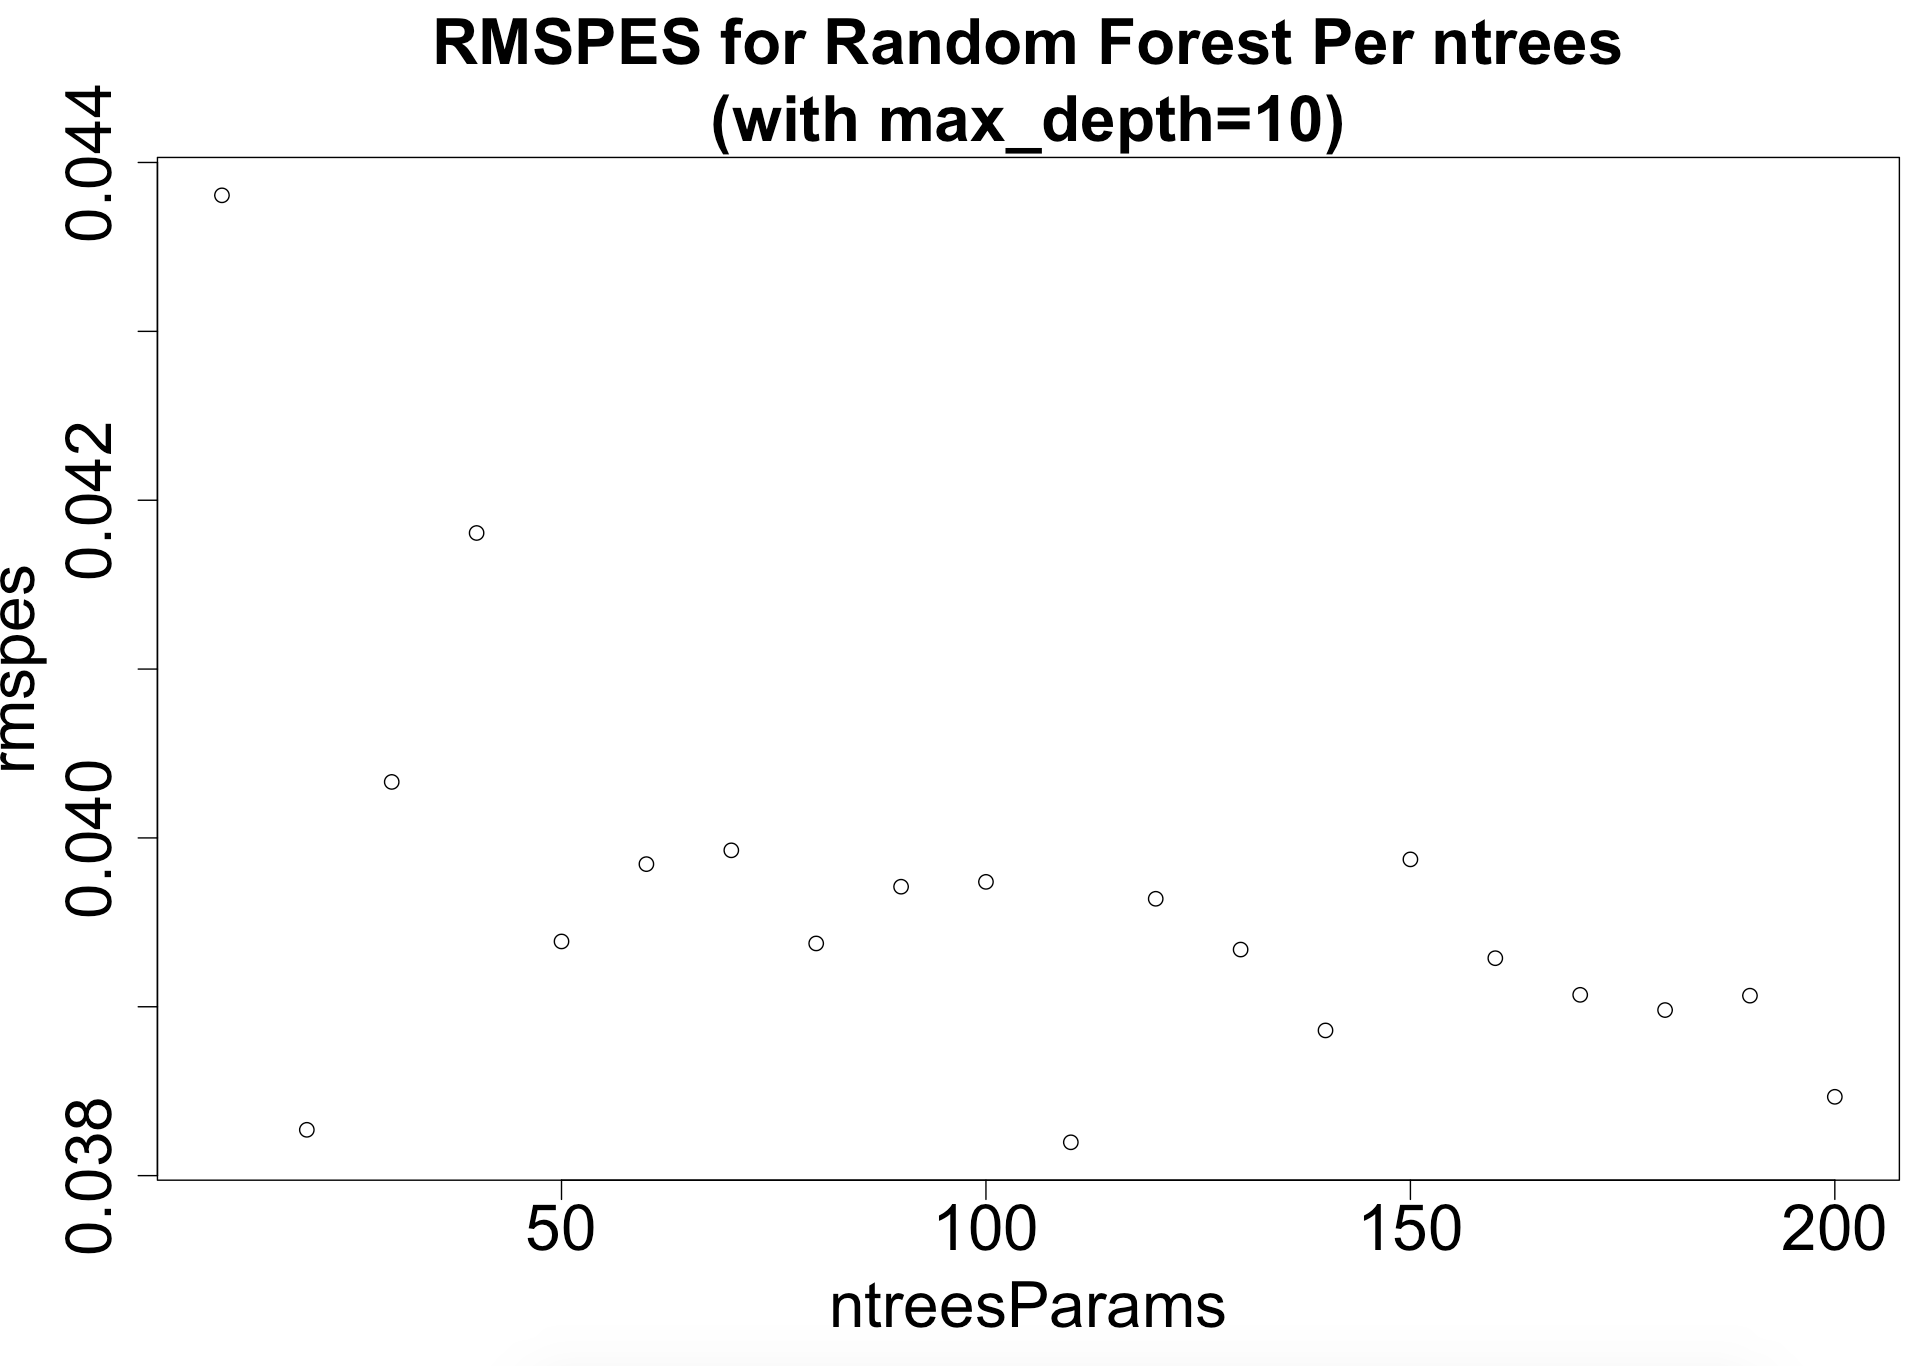
\includegraphics[scale=0.22]{img/RandomForestPerNtrees.png}

We see that, unlike the depth of trees, the number of trees parameter does not have much impact on RMSPE.

Hence, we chose 30 as depth, 100 as ntrees to run random forest. The error rate for random forest (depth=30, ntrees=100) was 0.020639 for validation set and 0.14411 on test set.

\subsection{Gradient Boosting}
Before comparing the results of gradient boosting with other algorithms we performed, let's explore on the results of gradient boosting itself only. Although we already feature engineered our data set, we decided to also see how our test error rate changes when we exclude stores with 0 sales. As we did in previous methodologies, we tried a range of certain parameters to maximize its prediction accuracy. Since the major issue of all machine learning tasks is to prevent overfitting on training data, we also used 5-fold cross validation to generalize. We computed the average error rates of 5-fold as a parameter changes, and graphed them to choose the best parameter. There are actually more parameters to tune in Gradient Boosting. There are three major parameters subject to be tuned: the step size of each boosting step (learning rate), maximum depth, and the max number of iterations. For our task, we decided to use the default number of trees and max number of iterations, but tune the step size. We might check how the different number of iterations affect the performance, but we checked it did not affect much but exponentially increase its runtime. We decided to set it as 300, and try different step sizes. 

The effects of tuning the step size are visualized in the following graph:

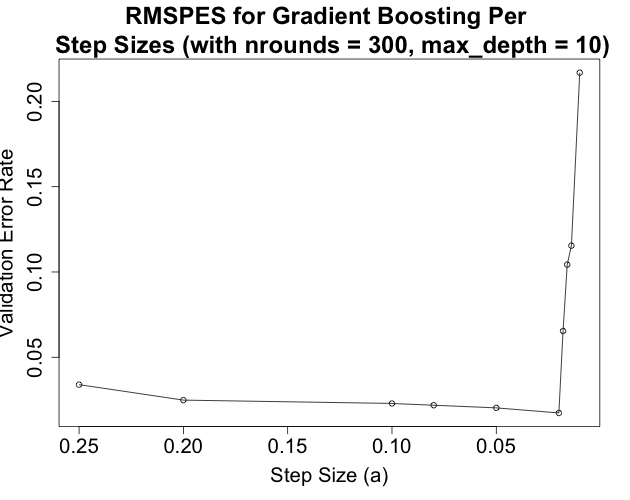
\includegraphics[scale=0.33]{img/gb_rmpse.png}

As the error rate shows, Gradient Boosting model gives us the most predictive power by far. We were able to achieve test error rate (RMPSE) of 0.13234.


\section{Discussion}
To visualize the overall performance of our different models, we organized the resulting error rates into a simple table. 

The error rates of our different models on validation and test sets are the following:

\begin{center}
    \begin{tabular}{| l | l | l |}
      \hline
       & Validation & Test \\ \hline
      Benchmark & 0.106209 & 0.25789  \\ \hline
      Linear Regression \\
      (Full Model) & 0.09101 & 0.21036 \\ \hline
      Linear Regression \\
      (Backward Elimination) & 0.09108 & 0.20988 \\ \hline
      Linear Regression \\
      (AIC) & 0.091006 & 0.21039 \\ \hline
      Random Forest & 0.020639 & 0.14411  \\ \hline
      Gradient Boosting & 0.01734 & 0.13234  \\ \hline
      \hline    
    \end{tabular}
\end{center}

    Although we readily outperformed our benchmark, as we expected, linear regression model did not perform very well because of the non-linearity of the data. However, we checked the sharp increase from linear regression to Random Forest model. we confirmed that tree based models can approximate functions with any ``non-linear shape'', whereas linear models can produce functions with a ``linear shape'' with respect to a chosen set of features. 

    There were 5 features removed by our feature selection of partial t-test which are ``Promo2SinceYear'', ``CompetitionOpenSinceMonth'',``Promo2'', ``CompetitionDistance''. This seems very reasonable that these variables had very low correlation coefficient with ``Sales'' variable when we computed correlation coeffcients between all the variables in Explanatory Data Analysis parts. Stepwise method also equally removed these features. Also, as we checked ``Promo1'', ``Open'',``DayOfWeek'',``month'' highly correlated with ``Sales'', their t-stats were also significant. 

    As a result, we were able to achieve 0.13234 test error rate using gradient boosting to predict Rossmann drugstore sales. Although boosting performed very well for this dataset, we witnessed it's harder to tune parameters and took longer time to train the data compared to Random Forest. While the number of tree is only usually tuned to train Random Forest, Gradient Boosting model requires several more parameters to be well-tuned. In addition, tuning such parameters and comparing corresponding performances requires much more time than computing Random Forest algorithm. Also, Random Forest does not easily overfit. Often, many statisticans including Breiman claim Random Forests does not overfit. We actually checked that our validation error rate of Random Forest did not increase back up (due to overfitting) as the number of trees increases (Breiman). However, Boosting algorithm is more robust to overfitting because it relies on every single data point and tries to find optimal linear combination of regression trees given the train dataset. Thus, it requires proper tuning to avoid such problem. 
    With regard to training time duration, for one round of cross validation, linear model took less than 2 minutes, Random Forest around 30 minutues, and Gradient Boosting around 50 minutes. For the Gradient Boosting model, it took more than 9 to 10 hours to finish whole cross validations to compute all the average validation error rates for its varying parameters, while Random Forest took only about 4-5 hours. We could have potentially increased the size of the number of tree and achieve better precision, at the risk of overfitting and longer training time which is a tradeoff between time and accuracy. In the future, it will be more helpful for us to train Gradient Boosting in any parallel computing environment or Amazon EC2 to expand our computing capacity. In that way, we believe we can find the best combination of parameters of Gradient Boosting in a reasonable amount of time. Also, even if the Rossmann Sales data is consecutive in time since the year 2013, we did not take account for this fact. We believe it is also worth trying to see how time series model would help us to increase our predictive power. 
In conclusion, we can check that our well-tuned gradient boosting model outperformed Random Forest. 

\section{References Cited}

Adriansson, Nils et al. “Forecasting Gdp Growth, or How Can Random Forests Improve Predictions in Economics?.” (2015).

Aiello, Spencer. ``Package ‘h2o'.'' Cran R-project. CRAN, 15 Mar. 2016. Web. 5 May 2016. $\langle$https://cran.r-project.org/web/packages/h2o/h2o.pdf$\rangle$.

Breiman, L., (2001a). ``Random Forests'', Machine Learning 45 (1) pp. 5-32.
R.D. https://www.diva-portal.org/smash/get/diva2:785776/\\
FULLTEXT01.pdf

Chen, Tianqi. ``Package ‘xgboost'.'' Cran R-project. CRAN, 15 Feb. 2016. Web. 5 May 2016. $\langle$https://cran.r-project.org/web/packages/xgboost/xgboost.pdf$\rangle$.

Chen, Tianqi. ”Introduction to Boosted Trees.” (2014): n. pag. $\langle$https://homes.cs.washington.edu/~tqchen/data/\\
pdf/BoostedTree.pdf$\rangle$. University of Washington, 22 Oct 2014. Web. 5 May 2016.

Dehkordi-Vakil, Farideh. ``Multiple Regression Analysis.'' DS-533. Illionis, Macomb. Lecture.

Gu, Jay (Haijie). ``Using Gradient Boosted Trees to Predict Bike Sharing Demand.'' Dato. 19 Aug. 2014. Web. 5 May 2016.

``Rossmann Store Sales.'' Rossmann Store Sales. Kaggle, 30 Sept. 2015. Web. 5 May 2016. $\langle$https://www.kaggle.com/c/rossmann-store-sales$\rangle$.

Mazerolle, Marc J. ``Making Sense out of Akaike’s Information Criterion.'' Avesbiodiv, Feb. 2007. Web. $\langle$ http://avesbiodiv.mncn.csic.es/estadistica/senseaic.pdf $\rangle$.

\section{Author Contributions}
Min Gu Jo and Wonjohn Choi closely collarborated together during the entire span of project, so they are well-aware of what each other have worked on. We believe that both of us contributed to this project equally.

Min Gu Jo contributed the followings:
\begin{itemize}
\item Wrote part of R codes in ``Section A: Pre-processing'' of ``final-project.R''.
\item Wrote R codes in ``Section B: EDA'' of ``final-project.R''.
\item Wrote part of R codes in ``Section I: Random Forest'' of ``final-project.R''.
  \item Wrote R codes in ``Section J: Gradient Boosting'' of ``final-project.R''.
\item Wrote part of ``1 Abstract'' section of paper.
\item Wrote ``2 Introduction'' section of paper.
\item Wrote ``3.2 EDA (Exploratory Data Analysis)'' section of paper.
\item Wrote ``3.3 5-fold Cross Validation'' section of paper.
\item Wrote ``3.7 Random Forest'' section of paper.
\item Wrote ``3.8 Gradient Boosting'' section of paper.
\item Wrote ``5.3 Random Forest'' section of paper.
\item Wrote ``5.4 Gradient Boostin'' section of paper.
\item Wrote ``7 Discussion'' section of paper.
  
\end{itemize}

Wonjohn Choi contributed the followings:
\begin{itemize}
\item Wrote part of R codes in ``Section A: Pre-processing'' of ``final-project.R''.
\item Wrote R codes in ``Section C: Utility Functions'' of ``final-project.R''.
\item Wrote R codes in ``Section D: Cross Validation'' of ``final-project.R''.
\item Wrote R codes in ``Section E: Benchmark'' of ``final-project.R''.
\item Wrote R codes in ``Section F: Linear Model'' of ``final-project.R''.
\item Wrote R codes in ``Section G: Variable Selection-Backward Elimination'' of ``final-project.R''.
\item Wrote R codes in ``Section H: Variable Selection-AIC'' of ``final-project.R''.
  \item Wrote part of R codes in ``Section I: Random Forest'' of ``final-project.R''.
  
\item Wrote part of ``1 Abstract'' section of paper.
\item Wrote ``2.1 Description of Datasets'' section of paper.
\item Wrote ``3.1 Preprocessing'' section of paper.
\item Wrote ``3.4 Error Metric'' section of paper.
\item Wrote ``3.5 Benchmark'' section of paper.
\item Wrote ``3.6 Linear Regression'' section of paper.
\item Wrote ``3.6.1 Feature Selection'' section of paper.
\item Wrote ``3.6.2 Feature Selection-Backward Elimination'' section of paper.
\item Wrote ``3.6.3 Feature Selection-Akaike Information Criterion'' section of paper.
\item Wrote ``4 Supplementary Methods'' section of paper.
\item Wrote ``5.1 Benchmark'' section of paper.
\item Wrote ``5.2 Linear Model'' section of paper.
  
  
\end{itemize}

\end{document}
